%% ============================================================
% f2012_shandong_arts_q16_rolling
%% f2012_shandong_arts_q16_rolling.tex
%% ============================================================
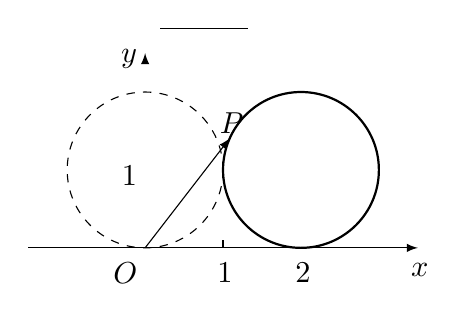
\begin{tikzpicture}[x=1bp,y=-1bp,
  every node/.style={inner sep=0,font=\fontsize{10.5pt}{12.6pt}\selectfont},
  line cap=butt, line join=miter]
  \draw[line width=0.42bp] (45.957,3.996) -- (77.445,3.996);
  \draw[line width=0.398bp] (-1.547,83.055) -- (135.133,83.055);
  \fill[black] (138.719,83.055) .. controls (137.656,82.855) and (135.93,82.258) .. (134.734,81.562) -- (134.734,84.547) .. controls (135.93,83.852) and (137.656,83.254) .. (138.719,83.055);
  \fill[black] (40.535,12.922) .. controls (40.336,13.984) and (39.738,15.711) .. (39.039,16.906) -- (42.027,16.906) .. controls (41.332,15.711) and (40.73,13.984) .. (40.535,12.922);
  \draw[line width=0.797bp] (68.586,83.055) -- (68.586,80.25);
  \draw[line width=0.797bp] (124.691,55.004) .. controls (124.691,39.508) and (112.133,26.949) .. (96.641,26.949) .. controls (81.145,26.949) and (68.586,39.508) .. (68.586,55.004) .. controls (68.586,70.496) and (81.145,83.055) .. (96.641,83.055) .. controls (112.133,83.055) and (124.691,70.496) .. (124.691,55.004) -- cycle;
  \draw[line width=0.398bp] (40.535,83.055) -- (68.816,46.434);
  \fill[black] (71.012,43.594) .. controls (70.203,44.312) and (68.672,45.312) .. (67.391,45.836) -- (69.758,47.66) .. controls (69.938,46.289) and (70.52,44.555) .. (71.012,43.594);
  \draw[line width=0.398bp, dash pattern=on 2.989bp off 2.989bp] (68.586,55.004) .. controls (68.586,39.508) and (56.027,26.949) .. (40.535,26.949) .. controls (25.039,26.949) and (12.48,39.508) .. (12.48,55.004) .. controls (12.48,70.496) and (25.039,83.055) .. (40.535,83.055) .. controls (56.027,83.055) and (68.586,70.496) .. (68.586,55.004) -- cycle;
  \node[anchor=base west] at (31.66,16.23) {$y$};
  \node[anchor=base west] at (67.28,41.97) {$P$};
  \node[anchor=base west] at (31.94,60.47) {$1$};
  \node[anchor=base west] at (136.11,93.37) {$x$};
  \node[anchor=base west] at (66.33,95.61) {$1$};
  \node[anchor=base west] at (94.39,95.61) {$2$};
  \node[anchor=base west] at (28.89,96.02) {$O$};
\end{tikzpicture}
